\documentclass[11pt]{book}
\usepackage{palatino}
\usepackage{amsfonts,amsmath,amssymb}
% \usepackage{graphicx}


\ifx\pdftexversion\undefined
    \usepackage[dvips]{graphicx}
\else
    \usepackage[pdftex]{graphicx}
    \usepackage{epstopdf}
    \epstopdfsetup{suffix=}
\fi


\begin{document}

%%%%%%%%%%%%%%%%%%%%%%%%%%%%%%%%%%%%%%%%
% Problem Set 5
%%%%%%%%%%%%%%%%%%%%%%%%%%%%%%%%%%%%%%%%

\pagestyle{empty}
{\noindent\bf Spring 2021 \hfill Firstname M.~Lastname}
\vskip 16pt
\centerline{\bf University of Central Florida}
\centerline{\bf College of Business}
\vskip 16pt
\centerline{\bf QMB 6911}
\centerline{\bf Capstone Project in Business Analytics}
\vskip 10pt
\centerline{\bf Solutions:  Problem Set \#5}
\vskip 32pt
\noindent




\section{Histogram and Density of Log. Fly Reel Prices}

To begin visually analyzing the data, 
include plots of the density that were created last week.

\subsection{All Fly Reels Together}

Start with the log of prices because prices were skewed.
Figure \ref{fig:hist_dens_log_price} is
a histogram of the logarithm of fly reel prices, 
along with a rug plot and a kernel density estimate. 
%
\begin{figure}[h!]
  \centering
  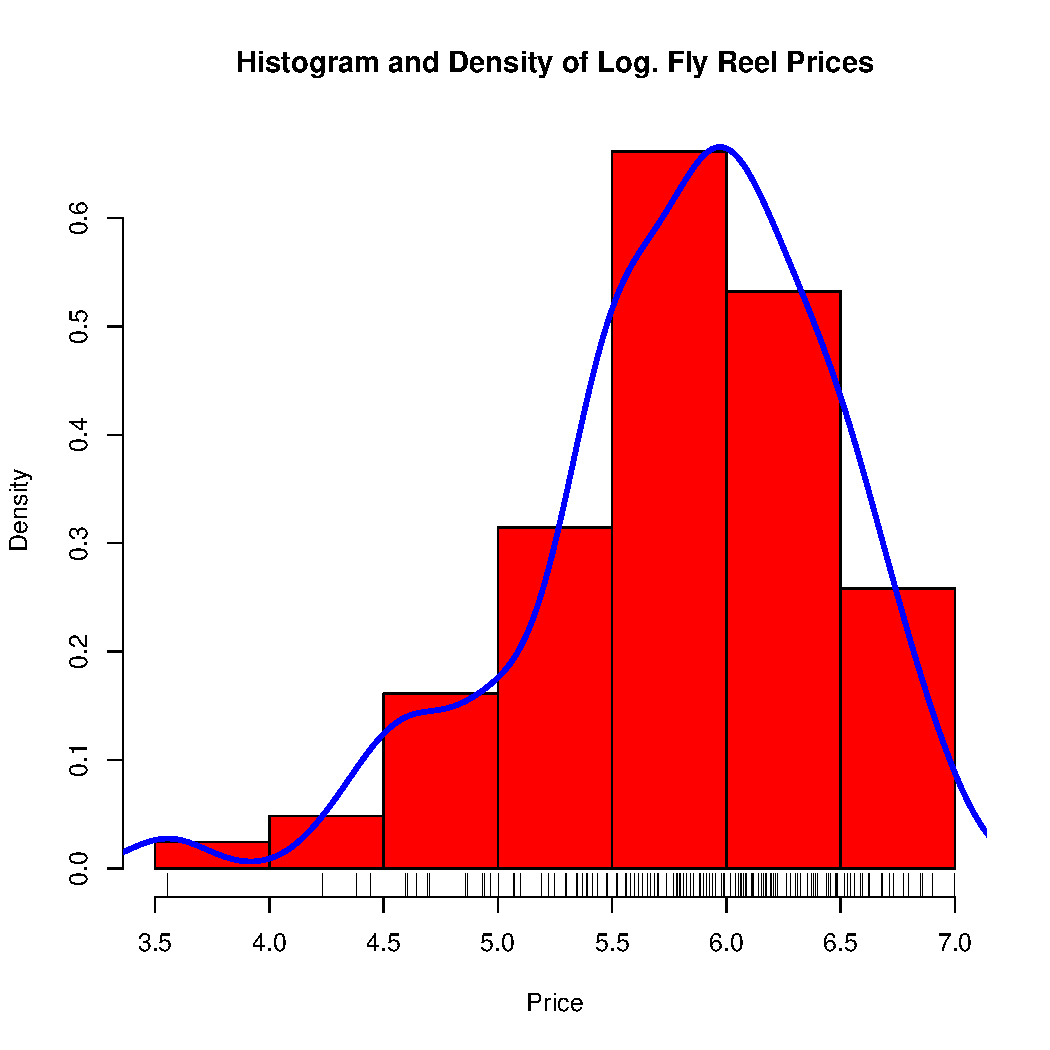
\includegraphics[scale = 0.5, keepaspectratio=true]{../Figures/hist_dens_log_price}
  \caption{Relative Histogram of Fly Reel Prices} \label{fig:hist_dens_log_price}
\end{figure}
% 
After taking logs, we can see that the distribution is
approximately symmetric, now with a slight skew to the left. 
Unlike the case of the tractors, 
the improvement from the log transformation is not so clear, 
so we should investigate this further in a later problem set. 


\clearpage
\pagebreak
\subsection{Comparison By Country of Manufacture}

Now we investigate the prices of fly reels made in the USA
compared to those made in China and Korea.
Figure \ref{fig:dens_by_country} shows the 
kernel density estimate of the prices of 
fly reels made in the USA in blue,
those made in China in red, 
and those made in Korea in green.
% 
The modes of the distributions are similar, 
however, we observe more variability in the prices of fly reels
made in Korea. 
The distribution of fly reels made in the USA is shifted 
toward the higher price range, compared to those made in other countries.
This indicates mild support for a ``Made in America'' premium
but we should also consider that it may be explained by 
the features of the reels made in the USA. 
We will investigate this further in regression analysis 
and other modeling approaches. 



\begin{figure}[h!]
  \centering
  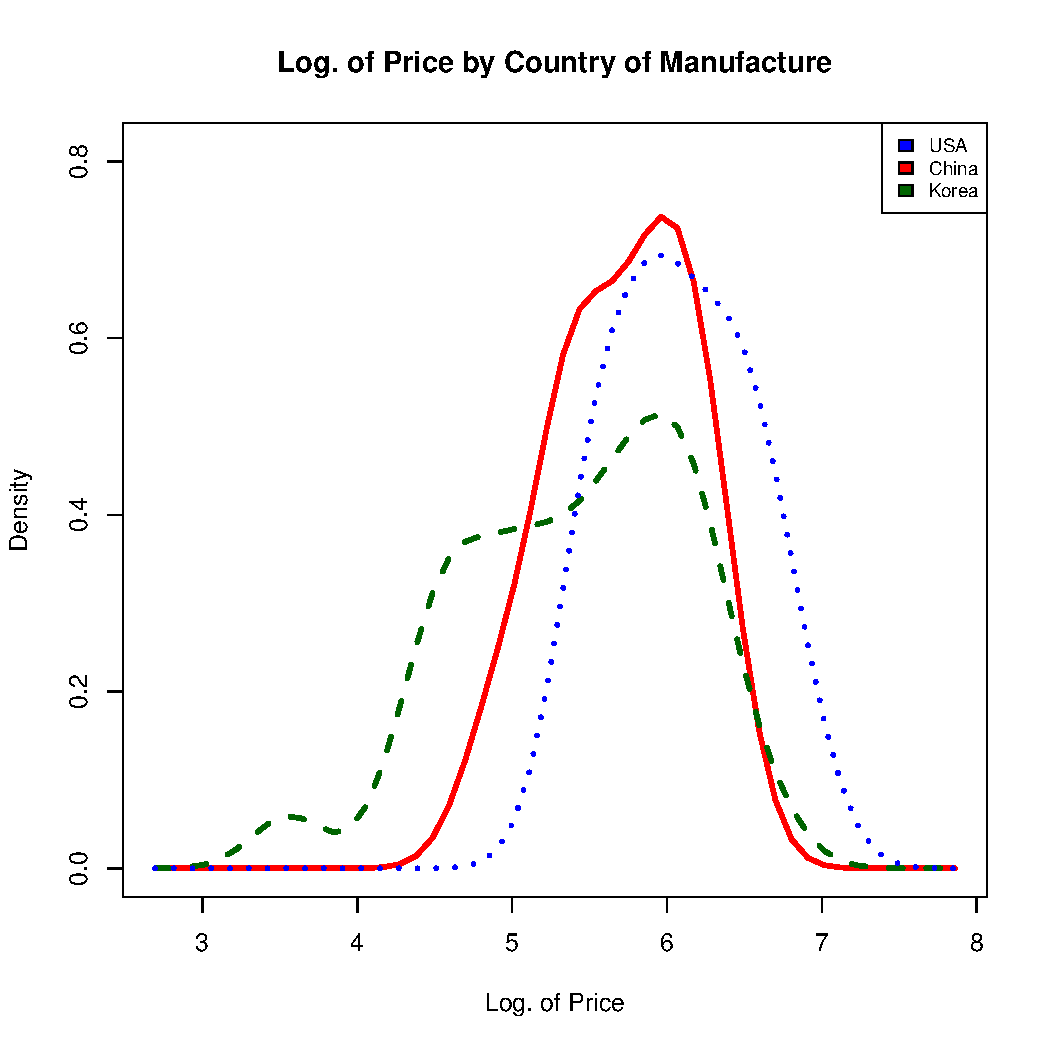
\includegraphics[scale = 0.5, keepaspectratio=true]{../Figures/dens_by_country}
  \caption{Densities of Log. Fly Reel Prices by Country of Manufacture} \label{fig:dens_by_country}
\end{figure}


\clearpage
\pagebreak
\section*{Scatterplot Matrices}


\subsection*{Scatterplots of Numeric Variables}

Figure \ref{fig:slpom_num_only} depicts a matrix of scatterplots
of the numeric variables in the dataset.

\begin{figure}[h!]
  \centering
  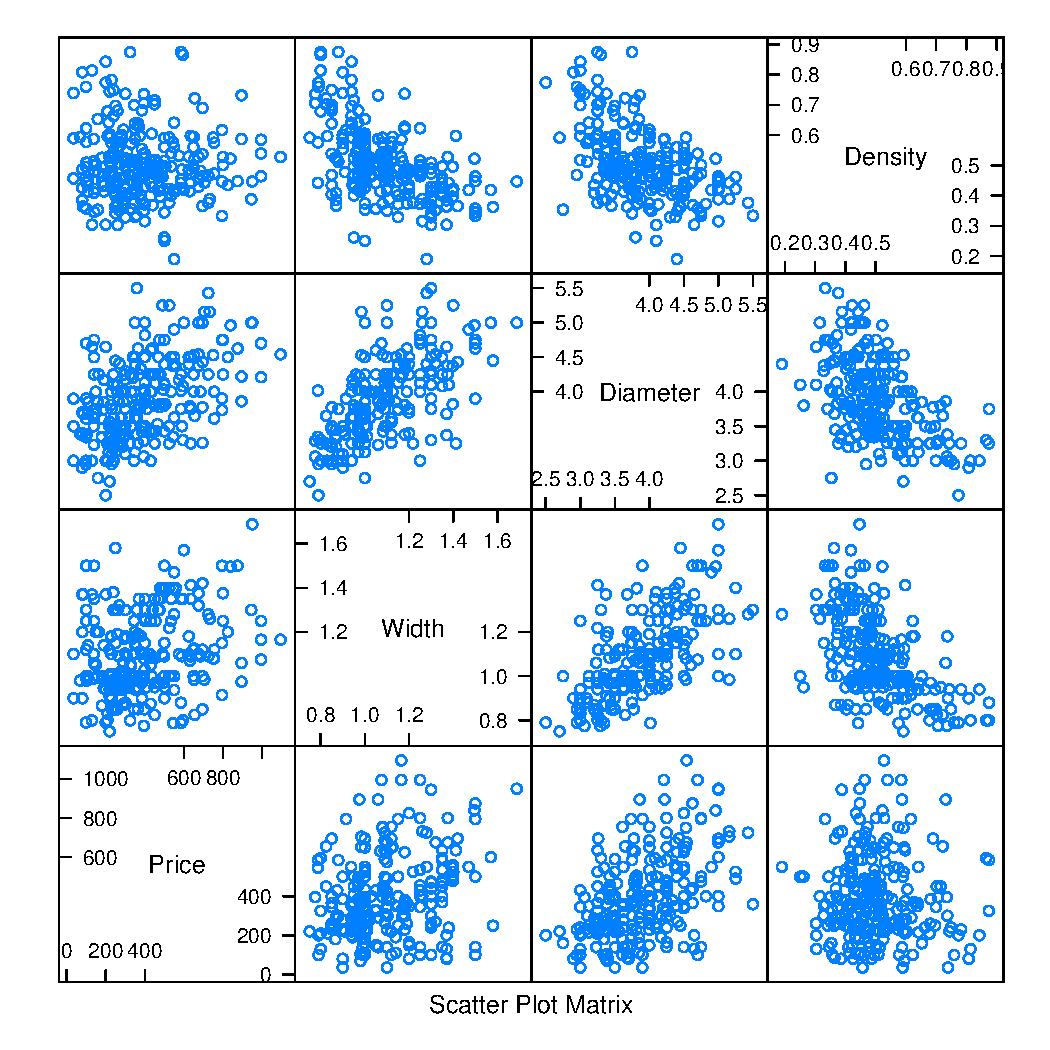
\includegraphics[scale = 0.5, keepaspectratio=true]{../Figures/slpom_num_only}
  \caption{Scatterplots of Numeric Variables} \label{fig:slpom_num_only}
\end{figure}


\pagebreak
\subsection*{Scatterplots with Categorical Variables}

Figure \ref{fig:slpom_with_cat} depicts a matrix of scatterplots
of with categorical variables in the dataset.

\begin{figure}[h!]
  \centering
  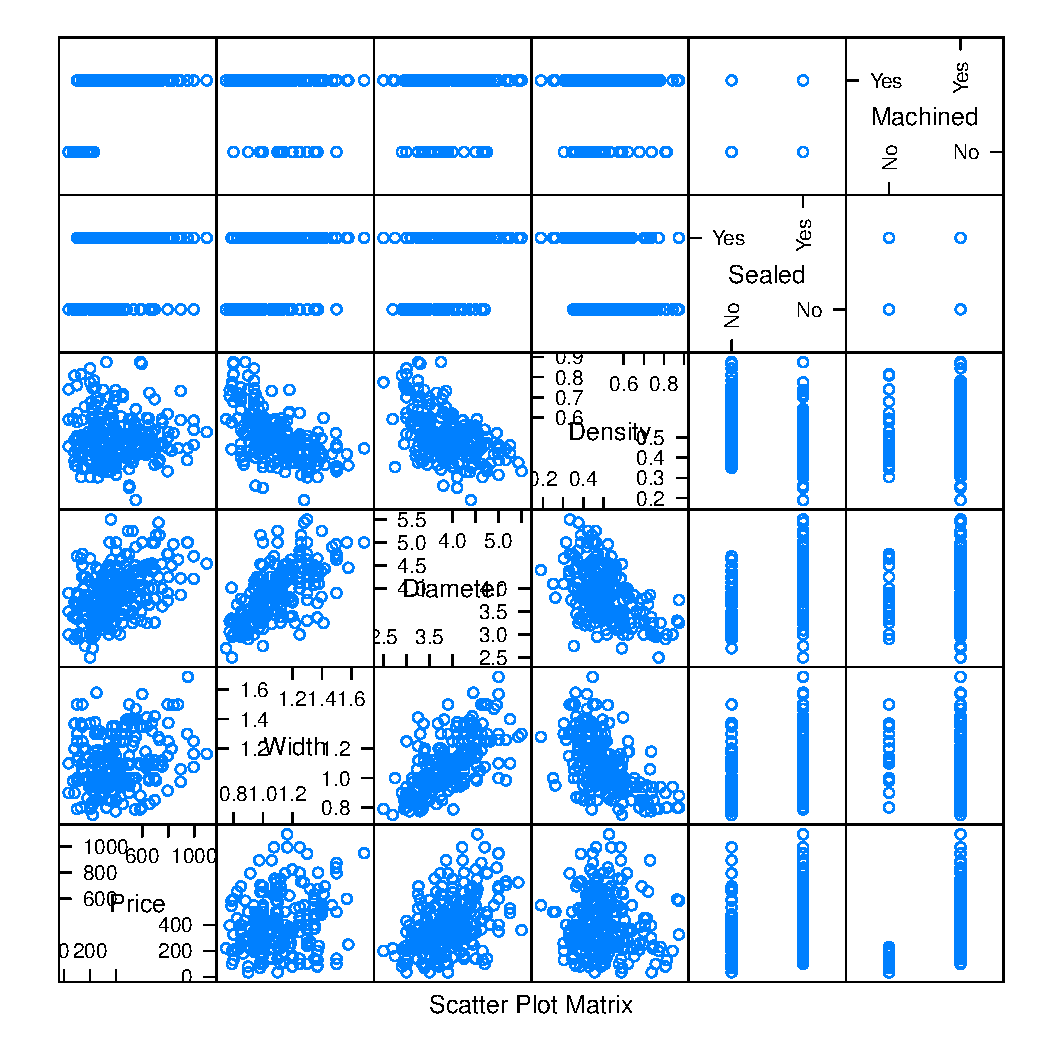
\includegraphics[scale = 0.5, keepaspectratio=true]{../Figures/slpom_with_cat}
  \caption{Scatterplots with Categorical Variables} \label{fig:slpom_with_cat}
\end{figure}


\pagebreak


Figure \ref{fig:slpom_with_sealed_mach.eps} depicts a matrix of scatterplots
with a categorical variable for the design combinations of the fly reels:
a fly reel is either sealed or unsealed and either machined or cast.

\begin{figure}[h!]
  \centering
  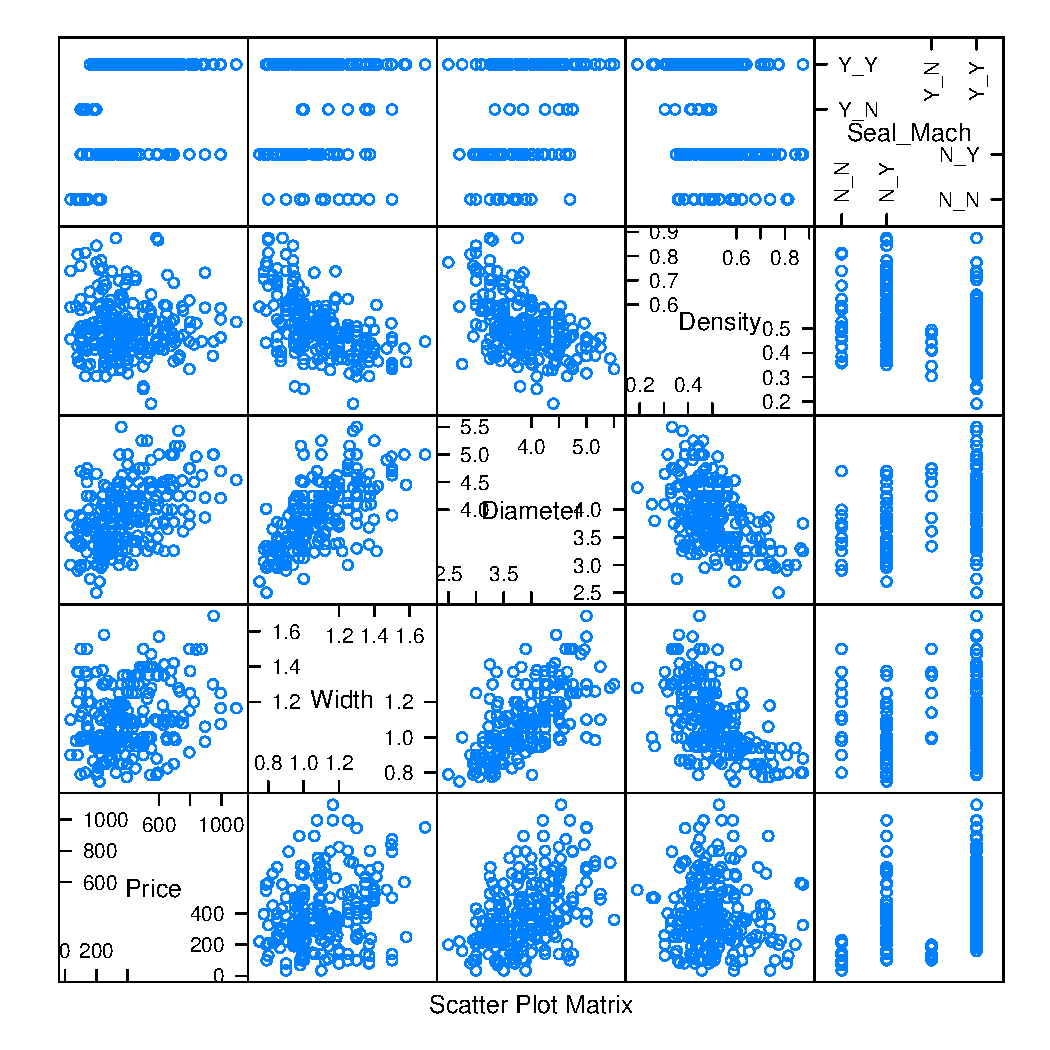
\includegraphics[scale = 0.5, keepaspectratio=true]{../Figures/slpom_with_sealed_mach.eps}
  \caption{Scatterplots of Numeric Variables} \label{fig:slpom_with_sealed_mach.eps}
\end{figure}



\pagebreak
\subsection*{Scatterplots by Country of Manufacture}

Figure \ref{fig:slpom_by_country} depicts a matrix of scatterplots
of the variables in the dataset
with the points indicated differently by country of manufacture.

\begin{figure}[h!]
  \centering
  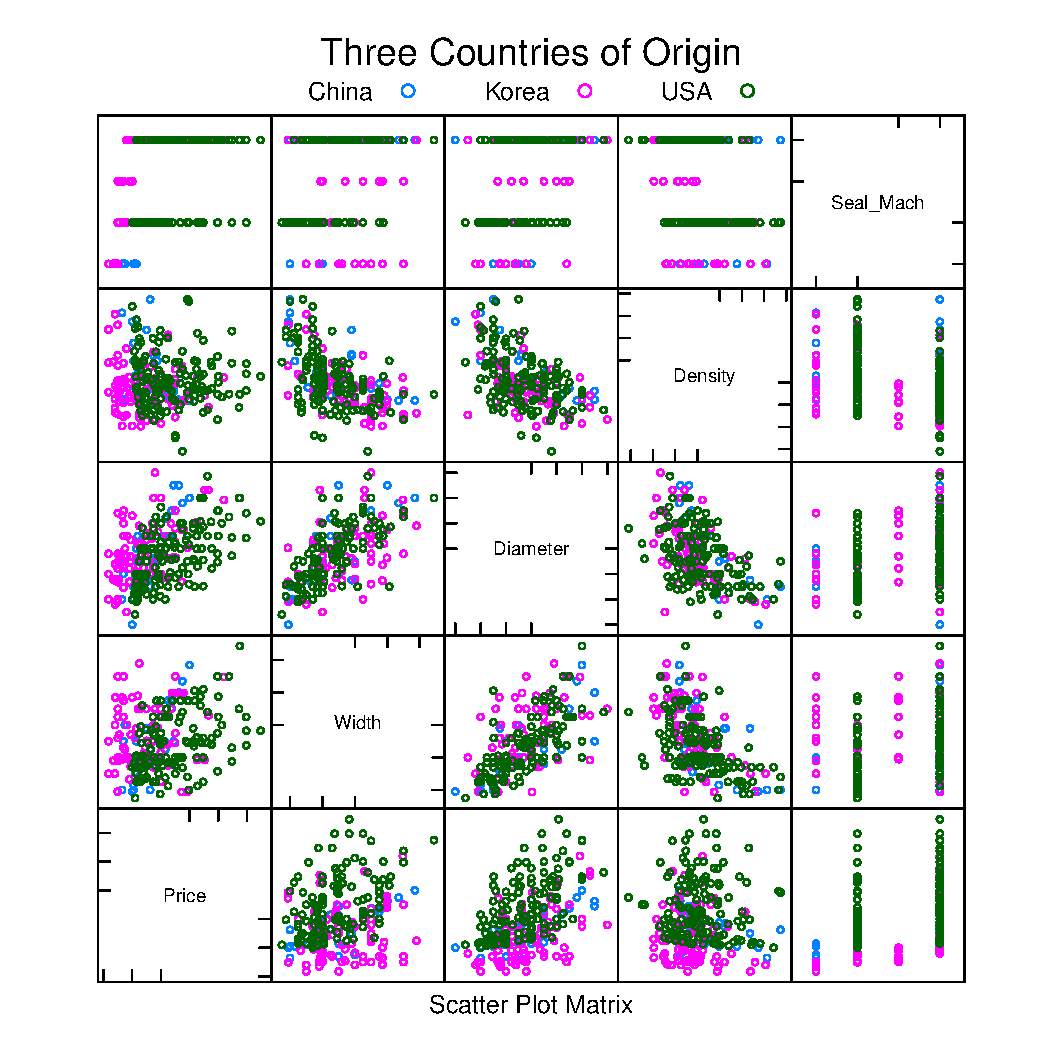
\includegraphics[scale = 0.5, keepaspectratio=true]{../Figures/slpom_by_country}
  \caption{Scatterplots by Country of Manufacture} \label{fig:slpom_by_country}
\end{figure}



\pagebreak
\subsection*{Dot Chart by Brand and Country of Manufacture}

Now consider the average prices by brand of fly reel and 
country of manufacture. 
Figure \ref{fig:dotchart_brand_country} depicts a dot chart
showing the average prices in the horizontal axis 
in these combinations of categories.


\begin{figure}[h!]
  \centering
  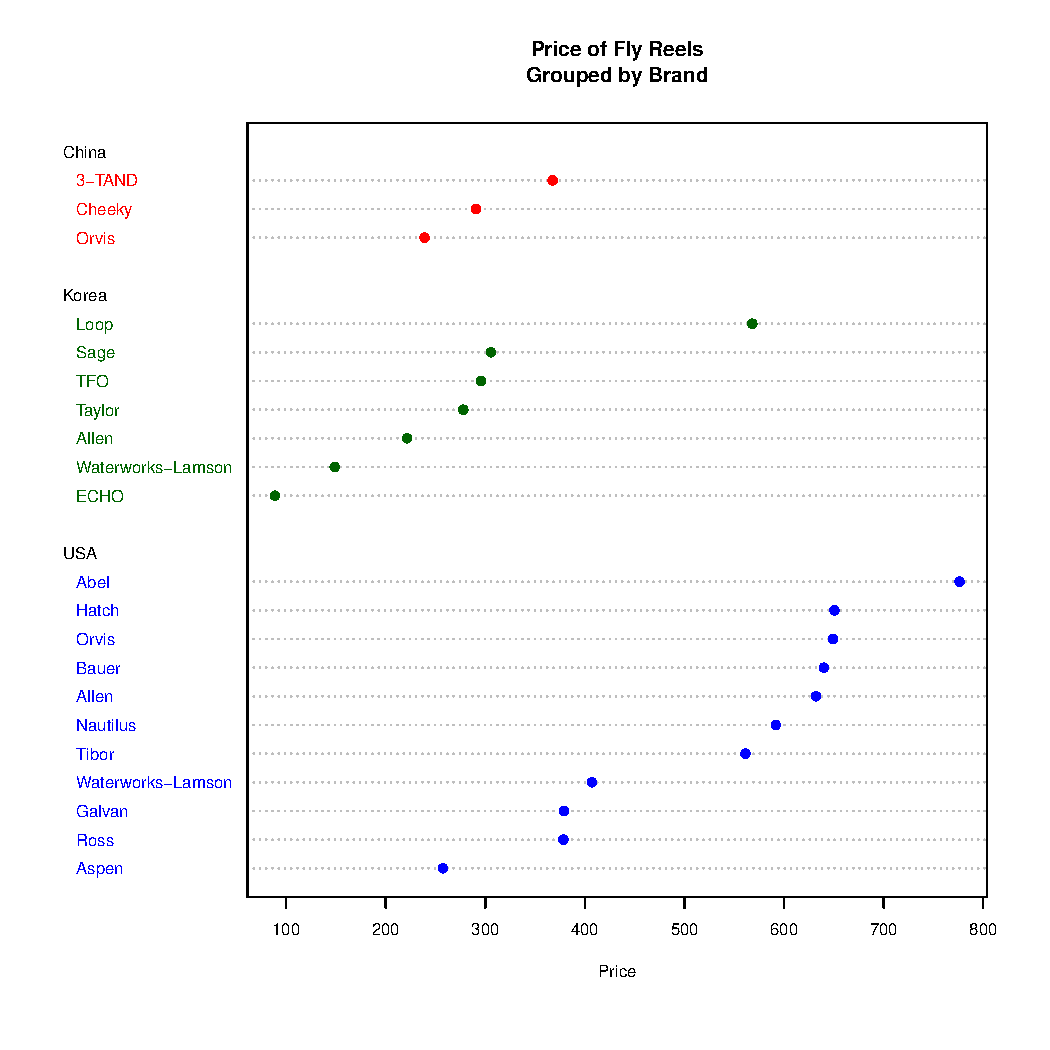
\includegraphics[scale = 0.5, keepaspectratio=true]{../Figures/dotchart_brand_country}
  \caption{Average Prices by Brand and Country of Manufacture} \label{fig:dotchart_brand_country}
\end{figure}

We see that there exists more variety, 
in terms of both the number of brands and price levels
within the population of American fly reel manufacturers. 
It's especially important that we consider the proliferation of 
fly reel brands at the high price points.
It is worth investigating further whether those fly reels
benefit from the ``Made in America'' premium
or are simply made with more valuable characteristics. 


%%%%%%%%%%%%%%%%%%%%%%%%%%%%%%%%%%%%%%%%
\end{document}
%%%%%%%%%%%%%%%%%%%%%%%%%%%%%%%%%%%%%%%%
